\documentclass[a4paper]{article}

% Caractères
\usepackage[utf8]{inputenc} % Codage des caractères en UTF-8
\usepackage[T1]{fontenc} % Fontes Extended Computer modern (EC)
\usepackage[french]{babel}
%\usepackage{lmodern} %  Fontes Latin Modern (LM)
%\usepackage{charter} % Police Charter
\usepackage{listings}

% Images
\usepackage{graphicx} % Inclure des images
\usepackage{float} % Placer les figures
%\usepackage{wrapfig} % Texte autour d'une image

% Format
% \usepackage{geometry} % Changer le format de la page
% \usepackage{pdflscape} % Changer le formate de la page

% En-tête et pieds de page
\usepackage{fancyhdr} % Inclure des en-têtes et des pieds de pages
\usepackage{lastpage} % Indiquer le nombre de pages du document

% Glossaire
\usepackage{glossaries} % Creer un glossaire

% Liens
\usepackage[unicode]{hyperref} % Inclure des liens externes
% \usepackage{url} % Inclure des URL

% Code
\usepackage{listings} % Inclure du code
% \usepackage{comment} % Commentaires sur plusieurs lignes

\title{Service - Boutique en ligne}
\author{Léo CASSIAU \and Geoffrey DESBROSSES}

\begin{document}

\maketitle

\section{Introduction}

    % Objectif perso
    Ce document résume le travail effectué au cours du projet de Service de 2\ieme{} année du master ALMA 2016 - 2017. Ce projet est mené par des étudiants de la faculté des sciences et techniques de Nantes, et le sujet est proposé par M. Redwene\footnote{\url{https://www.linkedin.com/in/redwene-haddou}}.
    
    \bigskip
    
    L'objectif de ce projet est de comprendre comment fonctionne la gestion de services dans une application. Pour cela, nous avons dû développer une application avec une certaine architecture qui permet d'exposer et de consommer des services facilement. L'architecture imposée est le Domain Driven Design (DDD). Le DDD est centré sur le métier de l’application et le code source qui l’implémente. Concrètement, le DDD est réparti en cinq couches qui ont chacune leur rôle à jouer dans l'application, mais il ne faut pas réfléchir technique mais plutôt à comment la technique peut permettre de réaliser mon problème. Pour cela il faut définir les actes métier et construire le projet autour de ça.

    \bigskip
    
    Le sujet du projet est de construire une boutique en ligne utilisant cette architecture DDD. Cette boutique doit fournir des services en Simple Object Access Protocol (SOAP) et également utiliser des services existants. Elle doit notamment utiliser les services d'un calculateur de taux de change, d'un service validant les achats par CB, et d'un fournisseur. C'est ce fournisseur qui permet de remplir la boutique de nouveaux articles à vendre, et ce service est développé par une autre équipe formée d'Ugo Mahey et Jean-Christophe Guérin. 
    
    \bigskip
    
    Les principales problématiques que soulève ce sujet tournent autour de l'architecture DDD et de la notion de service. En effet, cette approche demande de bien comprendre les rôles de chaque couche afin de répartir le code, tout en prenant en compte les problèmes de dépendances. Le choix des technologies utilisés est également un enjeu, qui nécessite d'étudier les différentes possibilités afin de choisir la solution adaptée.
    
    \bigskip
    
    Ce document commence par présenter notre architecture et le travail effectué. Ensuite, une deuxième partie justifie nos choix d'implémentation. Enfin, une conclusion résume l'expérience acquise au cours de ce projet et les futurs améliorations envisageable pour notre projet.

\newpage

\section{Réalisation d'une boutique en ligne }
   L'application développée est une simple boutique en ligne qui propose des articles à des clients et qui demande ses produits chez un fournisseur. Face à ce problème, il nous a fallu réfléchir sur les actes métiers d'une boutique de ce genre. 
   
   \bigskip
   
   Ainsi, nous avons pu cibler le problème et répartir les fonctions de notre application selon notre architecture DDD. Nous avons donc créé nos cinq couches applicatives : le domain, l'infrastructure, la présentation, l'Api puis enfin l'application.

\subsection{La couche domain}
    La couche domain représente la couche métier. C'est ici que nous avons défini nos classes métiers ainsi que les interfaces des factories et des repositories. Pour une boutique en ligne, nous avons simplifié les choses et définis trois objets :
    
    \bigskip
    
    \begin{enumerate}
        \item Client : client de la boutique
        \begin{itemize}
            \item name
            \item firstname
            \item age
            \item email
            \item password
            \item cart
        \end{itemize}
        
        \item Article : article vendu par la boutique
            \begin{itemize}
            \item id
            \item name
            \item description
            \item price
            \item available
            \item type
        \end{itemize}
        \item Cart : panier d'un client
    \end{enumerate}
    
    \bigskip
    
    Un client est un acheteur potentiel de notre boutique, il est unique et est identifié par son email. Celui-ci possède les attributs cités précédemment, dont un panier qui est simplement une liste d'articles. Chaque client est identifié sur la boutique et peut interagir avec elle, donc il y a un client par personne réelle qui doit pouvoir s'authentifier et réaliser les actions possibles sur la boutique.
    
    \bigskip
    
    Un client peut également avoir le rôle d'administrateur. Dans ce cas, il peut également demander les services du fournisseur et récupérer ses produits pour alimenter la boutique.
    
    \bigskip
    
    Un article est un produit proposé par la boutique, unique et identifié par son id. L'attribut available permet de savoir s'il est disponible ou non, donc si un client l'a déja acheté et si la boutique n'en a pas recommandé au fournisseur.

    \bigskip
    
    Une fois les objets définis, nous avons décrit les actes métiers, donc écrit les fonctions possibles par nos objets. Pour un client, il est possible d'ajouter un article au panier, d'en supprimer, de vider le panier ou encore de valider son panier, donc acheter tout son contenu).
    
    
    \bigskip
    
    Une vraie boutique en ligne possède une base de données, la notre est gérée dans la couche infrastructure. Cependant, nous avons défini des interfaces pour notre factory et notre repository pour gérer l'implémentation dans la bonne couche. Pour gérer la persistance des données, nous avons suivi le pattern DAO, donc la couche domain possède les interfaces IDAO et IDAOFactory.
    
    
\subsection{La couche infrastructure}
    Comme dit précédemment, cette couche gère la persistance des données. Cette couche à une dépendance vers la couche domain, donc nous avons pu utiliser les objets métiers pour interagir avec eux. 
    
    \bigskip
    
    Dans notre cas, nous avons choisi de stocker nos données dans une base de données mySQL ou Derby (Les deux implémentations ont été développées). Pour ce faire, nous avons une classe Connexion qui permet de se connecter à notre base de données et d'avoir accès au singleton Connexion n'importe quand et n'importe où dans notre application.
    
    \bigskip
    
    Ensuite, nous avons dû implémenter les interfaces définies dans le domain, soit implémenter les classes DAO et DAOFactory. La première sert à définir les méthodes qui vont permettrent à nos objets d'interragir avec la base de données (soit les méthodes CRUD et List) et la deuxième permet de créer les objets qui vont interragir avec la base de données.
    
    \bigskip
    
    Concrètement, un va demander à la factory de créer les objets ClientDao, ArticleDao et TypeArticleDao qui vont ensuite pouvoir exécuter les méthodes de leurs classes respectives (CRUD).
    
    \bigskip
    
    Par exemple, la classe ArticleDao possède la méthode create(Article obj) qui permet d'ajouter un article à notre base de données après l'avoir acheté au fournisseur.
    
    \subsection{La couche présentation}
        
    Pour une boutique en ligne, cette couche représente simplement l'interface graphique. Celle-ci a été développée avec les technologies HTML, CSS (Bootstrap) et Javascript (AngularJS) comme nous pouvons le voir sur la figure \ref{ihm}.
    
    \begin{figure}[H]
    \centering
    \caption{Interface graphique de la boutique}
    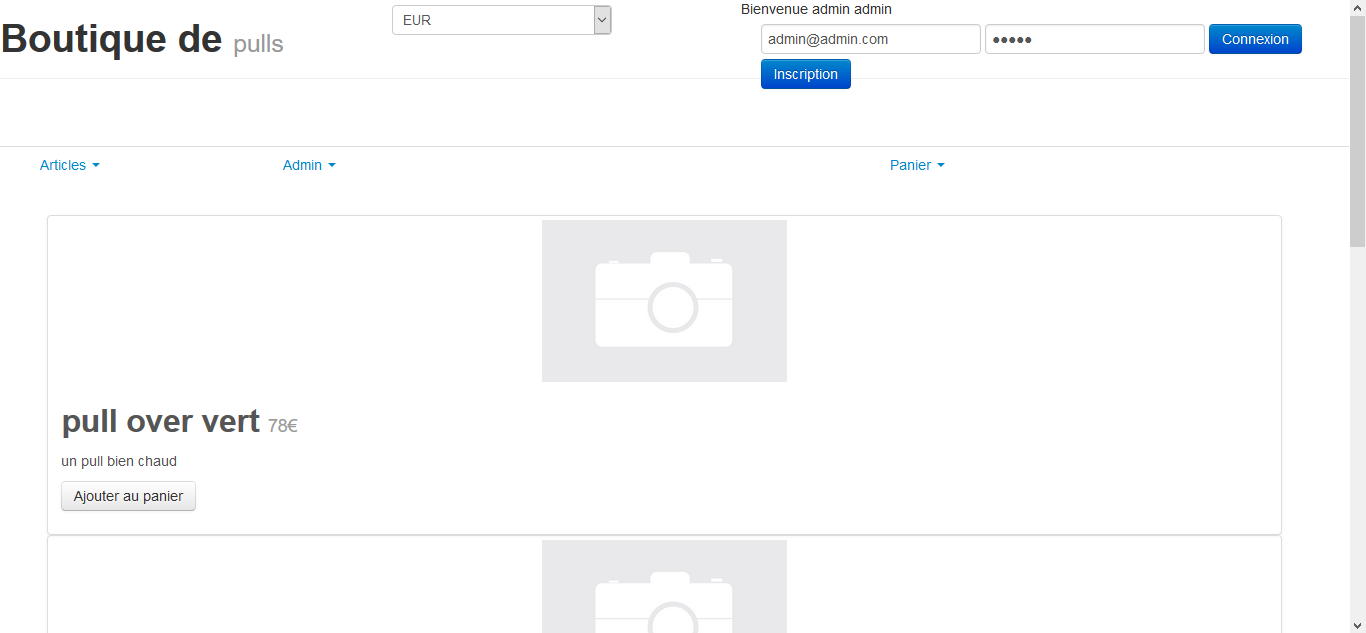
\includegraphics[width=\textwidth]{ihm.png}
    \label{ihm}
    \end{figure}
    
    \bigskip
    
    Les actions que peut réaliser un utilisateur sont afficher les articles par type, ajouter au panier, retirer du panier, vider le panier puis acheter le panier. Un administrateur peut lui ajouter un article à la boutique.
    
    \bigskip
    
    Ces actions sont réalisables en appelant les services distants de notre application. Pour cela, nous avons utilisé la librairie angular-soap permettant de faire des appels SOAP assez facilement. Il suffit juste de connaître l'url, le nom de la méthode distante puis ses paramètres.
    
\subsection{La couche Api}
    La couche Api est très importante dans une architecture DDD. C'est ici que l'on va définir les méthodes que l'on va proposer en tant que service. Cette couche n'a aucune dépendance, c'est juste un ensemble d'interfaces que l'on va devoir implémenter ailleurs pour écrire le corps des méthodes de service.
    
    \bigskip
    
    Notre application proposera donc les services suivants:
    
    \bigskip
    
    \begin{enumerate}
        \item Les services proposés à un client
        \begin{itemize}
            \item buy
            \item addToCart
            \item removeToCart
            \item clearCart
            \item getTypesArticles
            \item getArticles
            \item convert
            \item login
            \item signUp
        \end{itemize}
        
        \item Les services proposés au fournisseur
        \begin{itemize}
            \item buy
            \item getArticlesSupplier
        \end{itemize}
    \end{enumerate}
    
    \bigskip
    
\subsection{La couche application}
    
    La couche application connaît le domain ainsi que l'infrastructure. Elle peut donc interagir avec les objets métier ainsi qu'avec la base de données. Cette couche va proposer des services SOAP en suivant les interfaces définies dans la couche Api. Toutes les actions qui nécessitent une demande du serveur vont être implémentées ici. La solution choisit pour exposer ces services et les décrire est détaillé à partir de la partie \ref{sec:choix}.
    
    \bigskip
    
    Certaines de ces méthodes nécessitent des paramètres, par exemple, pour avoir tous les articles d'un type d'article, il faut passer le type d'article en paramètre. Pour cela, tous nos paramètres sont des chaines de caractères que l'ont doit recevoir sous le format JSON. À partir de ce JSON reçu, nous construisons notre objet, traitons la demande puis retournons un résultat encore sous format JSON. Nous pouvons voir un exemple sur les figures \ref{requete} et \ref{reponse}.
    
    \begin{figure}[H]
        \centering
        \caption{Requete de getArticles}
        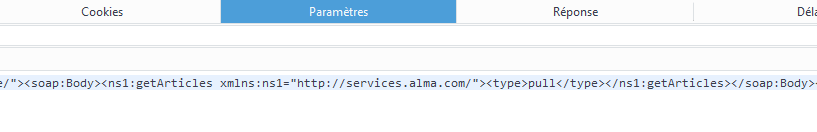
\includegraphics[width=\textwidth]{requete.png}
        \label{requete}
    \end{figure}
    
    \begin{figure}[H]
        \centering
        \caption{Reponse de getArticles}
        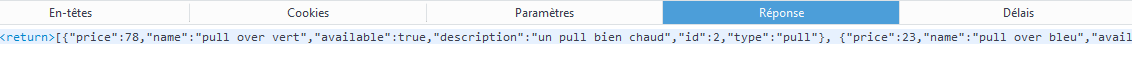
\includegraphics[width=\textwidth]{reponse.png}
        \label{reponse}
    \end{figure}
    
    C'est aussi dans cette couche que sont définies les actions qui n'ont aucun rapport avec le métier. Par exemple, c'est ici que sont définies les méthodes pour parser du JSON ou pour authentifier un utilisateur de la boutique.
    
    \bigskip
    
    Enfin, c'est dans cette couche que l'on consomme les services web externes, comme le service de taux de change. Nous avons utilisé le service disponible via le lien suivant \url{http://currencyconverter.kowabunga.net/converter.asmx} car il est simple d'utilisation et qu'il utilise SOAP comme demandé dans le sujet.

\section{Choix d'implémentation}
\subsection{Dépendance à l'Api}
    Dans notre application, il n'y a que l'application et le domain qui possèdent une dépendance vers l'Api. Nous envoyons nos données via des chaînes de caractères sous format JSON que nous parsons ensuite, donc tous nos paramètres sont des chaînes de caractères. C'est ensuite lors de l'implémentation de ces interfaces que nous décidons comment traiter la demande. Une fois la requête parsée, nous possédons nos vrais objets métiers et pouvons facilement interagir avec les couches domain et infrastructure. 
    
    \bigskip
    
    Par exemple, lorsque la présentation fait un appel SOAP pour ajouter un article au panier, l'application va recevoir une chaine de caractère de la forme suivante :
    
    \begin{lstlisting}
    {
        name : 'nom du client',
        firstname : 'prenom du client',
        age : 20,
        email : 'email@gmail.com',
        password : 'pass',
        cart : []
    
    },
    {
        id : 1,
        name : 'nom de l'article',
        description : 'description de l'article',
        price : 5,
        available : true,
        type : 'pull'
    }
    \end{lstlisting}
    
    \bigskip
    
    la méthode addToCart(String client, String article) va dans un premier temps parser le JSON reçu puis créer des vrais objets Client et Article en s'aidant de la couche domain et du parserJSON. Cette méthode va ensuite être capable d'appeler la méthode du domain permettant d'ajouter un article au panier de ce client et éventuellement de mettre à jour la base de données de l'infrastructure. C'est donc dans l'implémentation des services que l'on décide comment se comporte l'application.

\subsection{Dépendance de l'infrastructure} 
    L'infrastructure rentre des objets en base de données. Elle doit obligatoirement connaître les objets du domain pour savoir quels sont ses attributs. L'infrastructure implémente également la factory et le repository du domain, donc la dépendance vers le domain est très forte.
    
    \bigskip
    
    Cependant, l'infrastructure ne fait appel à aucune autre couche, ce n'est pas elle qui décide quand réaliser les actions, c'est plutôt l'application qui fait appel à l'infrastructure lorsqu'elle en a besoin.
    
\subsection{Choix de la base de données}
    Notre base de données contient la liste des clients et des articles à vendre. Nous avons décidé d'utiliser une base de données car ces données doivent être persistantes et peuvent devenir volumineuses. Dans un premier temps, nous avons utilisé MySQL comme serveur de base de données, mais son utilisation requiert d'installer MySQL au préalable. Nous avons donc décidé d'utiliser Apache Derby, pour une utilisation facilitée dans le cadre du projet. Derby permet de contenir les données dans un fichier tout en gardant le comportement SQL, et il peut être paramétré pour sauvegarder les données sur un serveur réel. L'utilisation de Derby avait pour principal but de faciliter le partage des données sur github et de réussir à faire fonctionner notre base de données sur les ordinateurs de la faculté. Nous avons gardé la classe établissant la connexion avec les serveurs MySQL afin d'intervertir leurs utilisations au besoin.

\subsection{Choix du serveur}\label{sec:choix}
    Nous avons choisi d'utiliser Tomcat 7 comme serveur pour exposer nos services. Nous avons opté pour cette solution car étant donné la petite taille de notre projet, son intégration est plus simple qu'un serveur d'application comme WSO2. En effet, un plugin est disponible sur maven, nous évitant de télécharger le serveur à chaque nouvelle installation. De plus, à l'aide de bibliothèques comme JAX-WS, cela nous permet de manipuler plus facilement les services et leur exposition ou non sur le serveur. Enfin, l'utilisation de tomcat7 permet de rendre plus rapide le déploiement des services suite à une modification, car nous n'avons pas besoin de passer par l'interface utilisateur de WSO2 pour rajouter le .jar.

\subsection{Traces des appels aux services}
    Le sujet du projet demandant de pouvoir obtenir les traces des appels des services, option disponible sur WSO2, nous avons choisi de créer des fichiers de logs résumant ces appels. Ces logs sont enregistrés côté serveur, et notifient la date, la classe, et le nom du service appelé. Nous avons utilisé log4j pour implémenter cette solution, qui se permet de mieux paramétrer les traces selon les besoins, et de manipuler facilement ces données pour d'éventuelles analyses.

\subsection{Structure des données échangés entre la présentation et l'application }
    Nous avons choisi d'utiliser le format JSON pour communiquer à l'aide des services, car il est facile à manipuler en AngularJS, plus lisible que le XML et il est de plus en plus populaire (ce qui présage un bon avenir).
    
\newpage

\section{Conclusion}

    Notre boutique en ligne est fonctionnelle. Elle possède plusieurs services qu'elle expose via des services SOAP et d'autres qu'elle consomme via le fournisseur. C'est une boutique en ligne qui ne possède pas beaucoup de fonctionnalités, mais celles qui sont essentielles sont présentes car nous avons réfléchis au métier avant tout.
    
    \bigskip
    
    Lors de ce projet, nous avons vu plusieurs aspects de la programmation et du travail d'un architecte logiciel. Maintenant, nous savons comment fonctionne une architecture à base de services car notre boutique en consomme et en expose. Nous comprenons également comment fonctionne une architecture Domain Driven Design. Ce type d'architecture est très pratique lorsque l'on souhaite diviser le développement en plusieurs couches. Il suffit simplement que chaque équipe suit les interfaces définies dans la couche API et d'implémenter sa couche avec les technologies et de la manière dont elle le souhaite.
    
    \bigskip
    
    Grâce à l'architecture de notre boutique en ligne, il est très facile d'ajouter de nouvelles fonctionnalités. Il suffit simplement d'ajouter un service dans l'API puis de l'implémenter dans chaque couche. De plus, toutes les couches (mis à part le domain) peuvent être jetées puis implémentées d'une autre façon, nous avons fait l'expérience lors de ce projet en migrant d'une base de données MySQL vers une base de données Derby, il a simplement fallu modifier la couche infrastructure. Il est également possible de modifier les autres couches, par exemple la présentation pourrait être implémentée en JEE à l'avenir. 
    
\end{document}
